%-------------------------------------------------------------------------------
\section{Introduction}
%-------------------------------------------------------------------------------

Web applications today own, store, and sell user data, often without the user's knowledge or
explicit consent~\cite{nytimes:fb, npr:data}. This can have dangerous consequences, with data leaks or
hacks~\cite{breach:twitter, breach:fb, breach:marriott, breach:quora} leading to loss of
livelihoods and lawsuits. Clearly, granting web applications complete data ownership fails to
protect users' privacy. To address this problem, laws such as the European Union's General Data
Protection Regulation (GDPR)~\cite{eu:gdpr} and California's Consumer Privacy Act
(CCPA)~\cite{ca:privacy-act} codify users' rights to data ownership, granting users the right to
request erasure of information related to them, and moving toward a world where user data 
ownership is fundamental and complete.

However, a world in which the user has complete data ownership is equally problematic.
Although feasible~\cite{amber, w5, blockstack, bstore}, this model results in an
arguably even less desirable world for users, leading to limited and slow applications, reduction of
useful service-side computation over shared data, and the requirement on users to maintain long-term
data storage themselves.  
\lyt{Not sure if we should mention the business model here, without addressing how you could charge
for user storage/application use, or how applications could be open-sourced and funded via
donations, etc.}
%Furthermore, such a model lacks a business model for
%companies to support applications of this nature.

This paper proposes a new model for web applications that balances users' desire for privacy with
their desire for application utility. In this model, users subscribe to applications by granting a
time-limited lease to their data, with the provision that the application may retain only
de-identified information once the user unsubscribes. Users can switch between a privacy-preserving
unsubscribed mode and an identity-revealing subscribed mode at any time without permanently losing
their data, or needing to maintain their account data themselves.  This model clearly benefits the
user: they can choose privacy at any time, without permanent loss of the application's storage and
utility benefits. But more importantly, the model benefits application developers as well: user data
can still be used to generate profit; the application retains less compromising data; and the
application supports the right to be forgotten while still allowing those users who leave to
easily come back. Figure~\ref{fig:world} illustrates this flexible transfer of data ownership in our
new model, as compared to the two extremes of complete user ownership and complete application
ownership of user data.

\begin{figure*}[ht!]
    \centering
    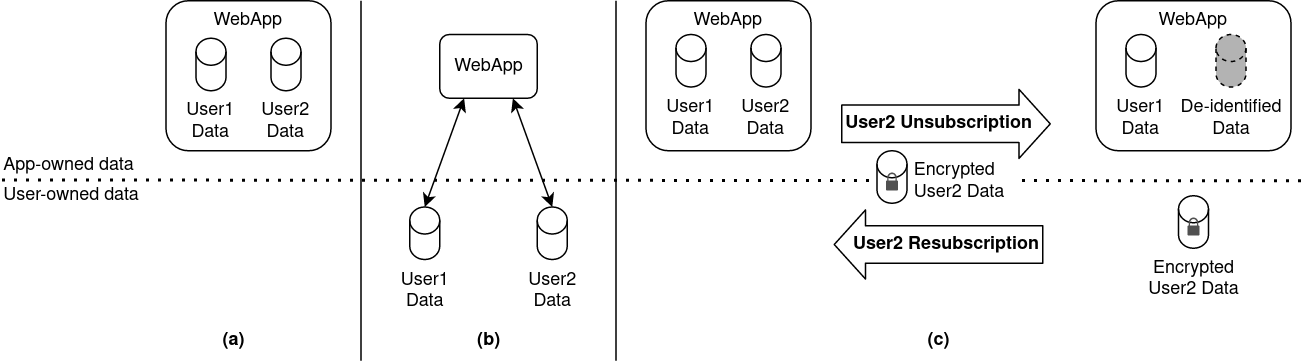
\includegraphics[width=\textwidth]{img/worlds}

    \caption{\textbf{(a)} The existing world of web applications, with applications maintaining and
    owning user data; \textbf{(b)} A world in which users have complete ownership of their data in cloud or local
    storage, and grant applications access to their data;
    \textbf{(c)} Our proposed model, which allows users to switch between privacy-preserving unsubscribed
    mode (right) and identity-revealing subscribed mode (left).}
    \label{fig:world}
\end{figure*}


Unfortunately, today's web services face many challenges that make free and easy unsubscription and
resubscription hard. Many do not support automated unsubscription, requiring users to 
contact the developers or customer support directly in order to unsubscribe.
Developers must manually implement unsubscription, leading to coarse-grained, error-prone data
handling that can fail to completely de-identify the user. Many applications require that some
information remains post-unsubscription, for legal or necessary application use, but retained data
can identify a user in complex ways: both user identifiers (\eg usernames) and structural
\emph{correlations} between application data records (\eg between users and posts, or posts and
tags) may reveal identifying information.  Without a systematic way to anonymize user identifiers
and \emph{decorrelate} these potentially identifying structural correlations, many developers have
chosen to either entirely delete all sensitive data at the expense of other subscribed users, or
leave identifying information unchanged at the expense of unsubscribed users.

Even if de-identification were easy, services that do provide some amount of de-identification upon
unsubscription fail to support resubscription, thus permanently deleting years or even decades of
accumulated application data. This permanent loss of user data costs both users and the web
service, and creates little incentive to lower barriers to unsubscription.  

The challenges and complexity of
correct unsubscription highlight the need for new tools that allow developers to easily and
systematically express how application data and structural correlations need to change when a user
unsubscribes, and support automatic resubscription and recorrelation of users with their account
data at any time.

In the rest of this paper, we describe the current support for unsubscription and resubscription in
today's web applications, and the challenges of implementing it correctly.  We then describe \sys, a
system that provides abstractions and mechanisms to help developers of databased-backed web
applications achieve correct, privacy-compliant user unsubscription and resubscription without
onerous labor, and without adding undue overheads.
